% !TeX spellcheck = cs_CZ
%{\tikzset{external/prefix={tikz/FYZII/}}
% \tikzset{external/figure name/.add={ch32_}{}}
%---------------------------------------------------------------------------------------------------
% file fey2ch32.tex
%---------------------------------------------------------------------------------------------------
%=========================== Kapitola Index lomu opticky hustých látek =============================
\setchaptertoc
\chapter{Index lomu opticky hustých látek}\label{fyz:IIchapXXXII}

  \section{Polarizace látky}\label{fyz:IIchapXXXIIsecI}
  \section{Maxwellovy rovnice v dielektriku}\label{fyz:IIchapXXXIIsecII}
  \section{Vlny v dielektriku}\label{fyz:IIchapXXXIIsecIII}
  \section{Komplexní index lomu}\label{fyz:IIchapXXXIIsecIV}
  \section{Index lomu směsi}\label{fyz:IIchapXXXIIsecV}
  \section{Vlny v kovech}\label{fyz:IIchapXXXIIsecVI}
  \section{Nízkofrekvenční a vysokofrekvenční přiblížení. Tloušťka skinové vrstvy a 
  plazmová frekvence}\label{fyz:IIchapXXXIIsecVII}
  \section{Příklady a cvičení}\label{fyz:IIchapXXXIIsecVIII}

    \begin{figure}[ht!] %\ref{fyz:fig871}
      \centering
      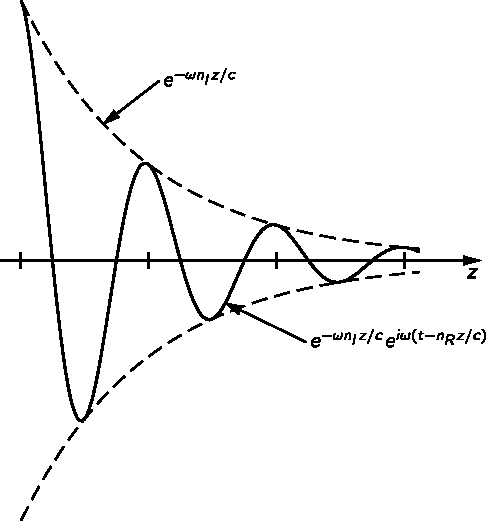
\includegraphics[width=0.7\linewidth]{fyz_fig871.pdf}
      \caption{
               (\cite[s.~707]{Feynman02})}
      \label{fyz:fig871}
    \end{figure}

    \begin{figure}[ht!] %\ref{fyz:fig872}
      \centering
      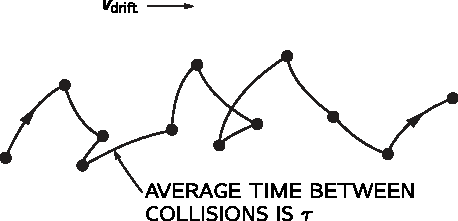
\includegraphics[width=0.7\linewidth]{fyz_fig872.pdf}
      \caption{
               (\cite[s.~707]{Feynman02})}
      \label{fyz:fig872}
    \end{figure}

    \begin{figure}[ht!] %\ref{fyz:fig873}
      \centering
      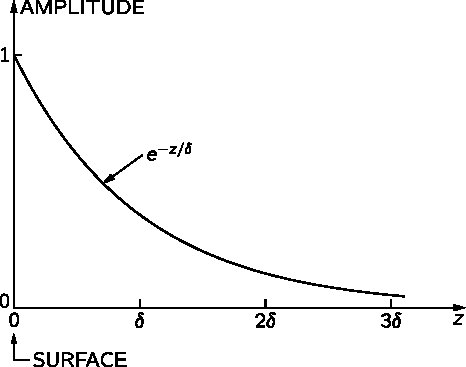
\includegraphics[width=0.7\linewidth]{fyz_fig873.pdf}
      \caption{
               (\cite[s.~707]{Feynman02})}
      \label{fyz:fig873}
    \end{figure}
 
    \todo[inline]{Kapitola fey2ch32 je nedodělaná, obsahuje pouze obrázky}
%} %tikzset
%---------------------------------------------------------------------------------------------------
